\chapter{Preliminary Results}

\section{Result Evaluation}

We evaluate our results using precision ($P$), recall ($R$) and the balanced F-measure ($F_1$) defined as follows:
\begin{align}
     P &= \frac{\mathit{TP}}{\mathit{TP} + \mathit{FP}}, \\
     R &= \frac{\mathit{TP}}{\mathit{TP} + \mathit{FN}}, \\  
     F_1 &= \frac{2 P R}{P + R}
\end{align}
where 
\acp{TP} is the number of pixels correctly marked as positive, 
\acp{FN} is the number incorrectly marked as negative and 
\acp{FP} is the number incorrectly marked as positive. 

We compare our results against common segmentation approaches \ac{SLIC}~\cite{Achanta:149300},
\ActiveContours{}~\cite{ActiveContou09} and \GrabCut{}~\cite{Rother2004-ou} in
Table~\ref{tab:quantitative-against-common} using a manually annotated region of Phoenix AZ. The
test region was acquired as \ac{VHR} 4-inch aerial orthophotos, and manually annotated by drawing a
polygonal outline. When a portion of the sidewalk was occluded or camouflage with the surrounding
pavement (including gutters) we used our best judgment to connect the visible portions of the
sidewalk. For all of of the examples we present we set $c_\mathit{bend}=\frac{1}{2},
c_\mathit{shrink}=c_\mathit{expand}=2$ which were experimentally found to produce the best result. 
Figure \ref{fig:change_on_recall} that shows detailed parameter evaluation for
 $c_\mathit{bend},c_\mathit{shrink}$, and $c_\mathit{expand}$. 
Note that in our implementation we did not take care to ensure that $\Pr(\delta_k)$ summed to unity,
and instead assumed that $-\lg \Pr(\delta_k=0)$ was zero, which does not have a probabilistic
interpretation but is more convenient for computation.

\begin{table}[h!]
    \caption{Quantitative comparison. }
    \label{tab:quantitative-against-common}
    \centering
    \begin{tabular}{r ccc}
                            & $P$ & $R$& $F_1$ \\ 
                                 \hline 
                  \ac{SLIC} & 0.876 & 0.839 & 0.857 \\
          \ActiveContours{} & 0.873 & 0.866 & 0.869  \\
                 \GrabCut{} & 0.969 & 0.877 & 0.925  \\ 
                                 \hline
                \textbf{DP} & \textbf{0.973} & \textbf{0.961} & \textbf{0.967}   
    \end{tabular}
\end{table}

For qualitative comparison we compare against \ac{SLIC}, \ActiveContours{}, and \GrabCut{}, in
\figref{fig:Sample_4_compare}. The former presents a portion of a hiking trail in a desert region where the foreground and background materials are similar and the path curves and varies in thickness. The \ac{DP} approach is smooth and also follows the boundary of the path closely, and it also follows a reasonable trajectory where the path bifurcates. More challenging scenarios are shown in \figref{fig:Sample_2_compare} and \figref{fig:Sample_3_compare}, which includes examples of occlusion, shadow, and camouflage.  

\begin{figure}[H]
    \centering
    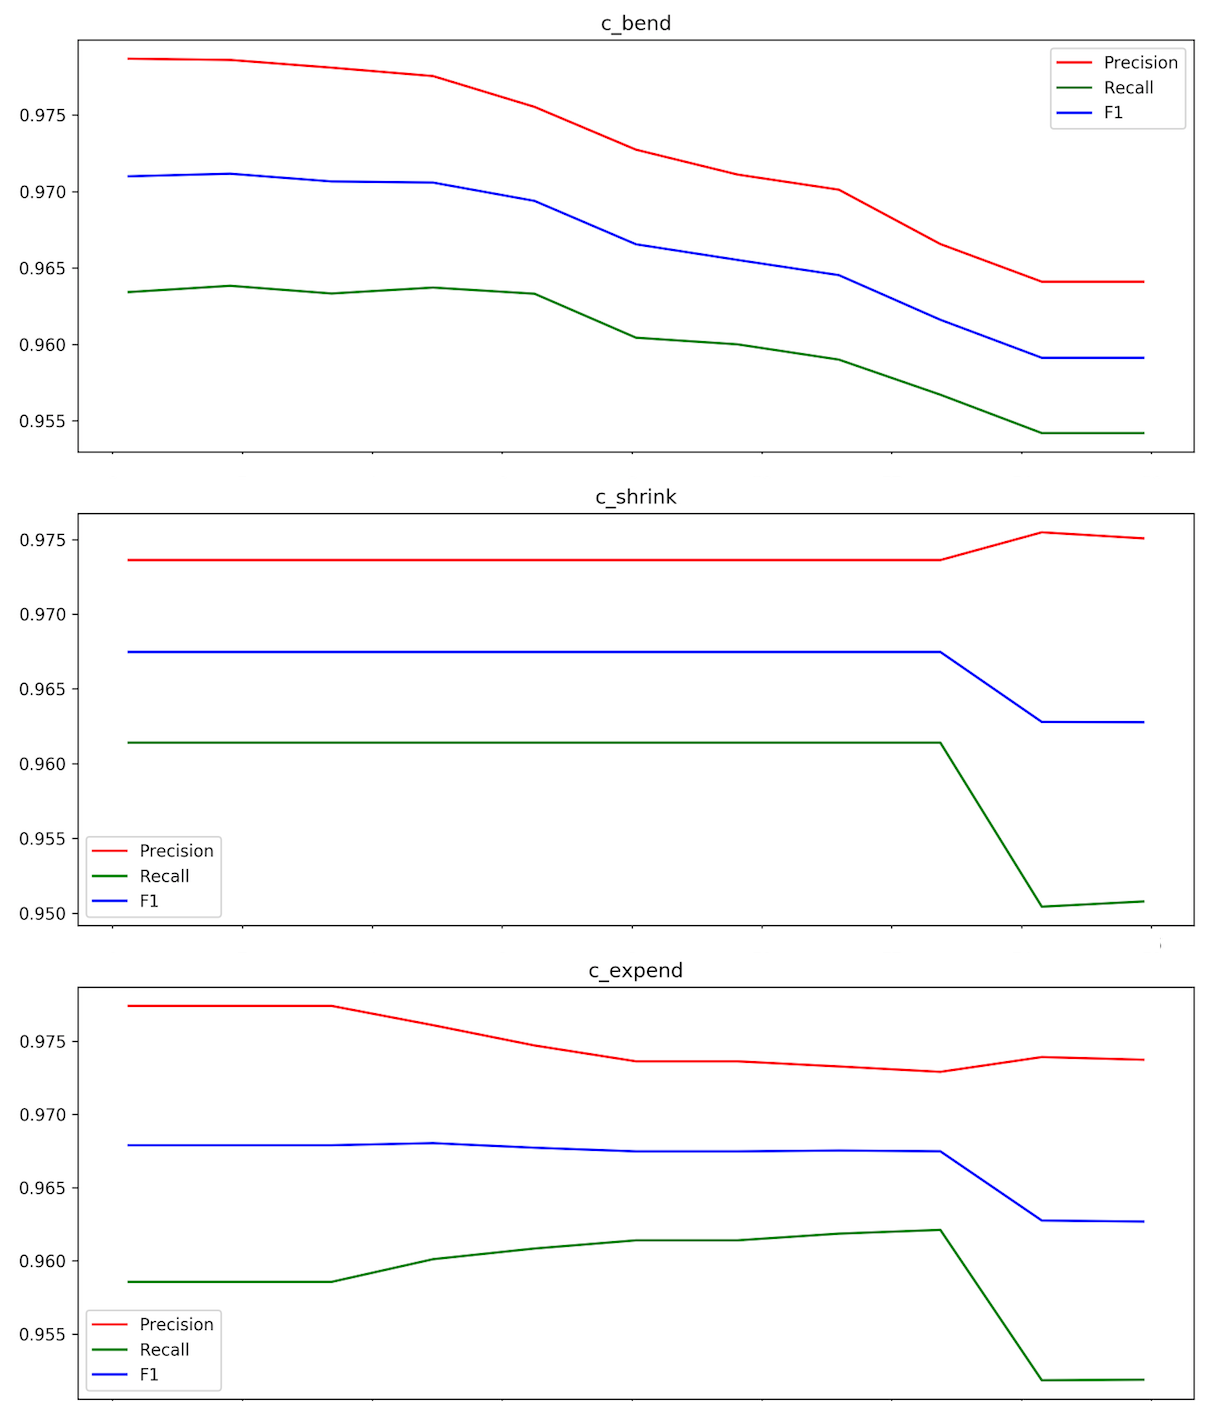
\includegraphics[width=0.65\textwidth]{Figures/prf.png}
    \caption[Parameters Evaluation]{Detail comparison on $c_{bend}$, $c_{shrink}$ and $c_{expand}$.
     Where red lines represent Recall, green lines represent Precision and blue lines represent F1.}
    \label{fig:change_on_recall}
\end{figure}

We have also identified the following limitations of the proposed method: it assumes that an initial ribbon overlaps with the feature in the corresponding orthophoto. 
We have not suggested an approach to determine if a walking path has been removed, or has been completely occluded. Furthermore, we assume \ac{VHR} orthoimagery that has enough resolution to build a model for colors on and off the ribbon. 
The proposed approach finds integer raddii, so thicknesses are all multiples of two. 
We recommend up-sampling images, which will allow the proposed approach to solve for a trajectory with sub-pixel precision. 
Finally, while we do make some assumptions when we select $\MinRadius{}, \MaxRadius{}, \MaxDistance{}$ the method as presented does not impose a prior on expected thickness of ribbons; often this is known and it could be used to generate plausible results for completely occluded ribbons.

We also test our approach in different cities. 
For initial trajectories, we pull the corresponding footway data from overpass-turbo \cite{overpass_turbo}.
Finding map data is challenging since there not exist much \ac{VHR} imagery from public source. 
We use the imagery data form GIS government database and treat it as input map. 
\figref{fig:oxford1} demonstrate plausible result on a sidewalks heavy area, we randomly selected a few from Oxford, OH. 
Row 1 shows that our approach are able to find the precise boundaries under trees or building shadows, with less accuracy around intersection area. 
Except above from row1, row 2 also demonstrate the camouflage with adjacent material. 
We treat the intersection part as overlapping sidewalks, and process them individually. \figref{fig:ny1} and \figref{fig:ny3} show the random samples we select from New York area. 
Predicting is heavier involved in these area since some sidewalks are partially under tree leaves instead of just shadows. 

% \todo[TALK ABOUT OTHER CITY]

% We generated few results from our sample inputs to compare with other methods according to figure \ref{fig:Sample_4_compare} and mathematics feedback from table \ref{table:sample_4}. From above feedback, Grabcut had decent performance with recognized edges for given sidewalk, since it's false positive (Red) in figure \ref{fig:Sample_4_compare} is significantly small. The problem that mentioned in chapter 2 is still the main reason that it's result is less accurate than ours. In row 1, 2, 3, column 1 of figure \ref{fig:Sample_4_compare}, the grabcut is unable to segment sidewalks which under the tree shadows. For the same issue, in column 4, our result indicated that we could successfully recognize and get boundaries from sidewalk. Same with figure \ref{fig:Sample_2_compare}. In row 1, 2, 3, we compared the output from column 1 and column 4, which are the outputs from grabcut and our approach. It's clear that our approach can successfully segment sidewalk when it connects with drive way (column 1), or there's obstacle (column 3) exist, not only for tree shadows. Also, another advantage of our algorithm is that our approach can segment sidewalks from gutters. We believe other methods are not able to recognize gutter under any circumstances. 

\begin{figure}[H]
    \centering
    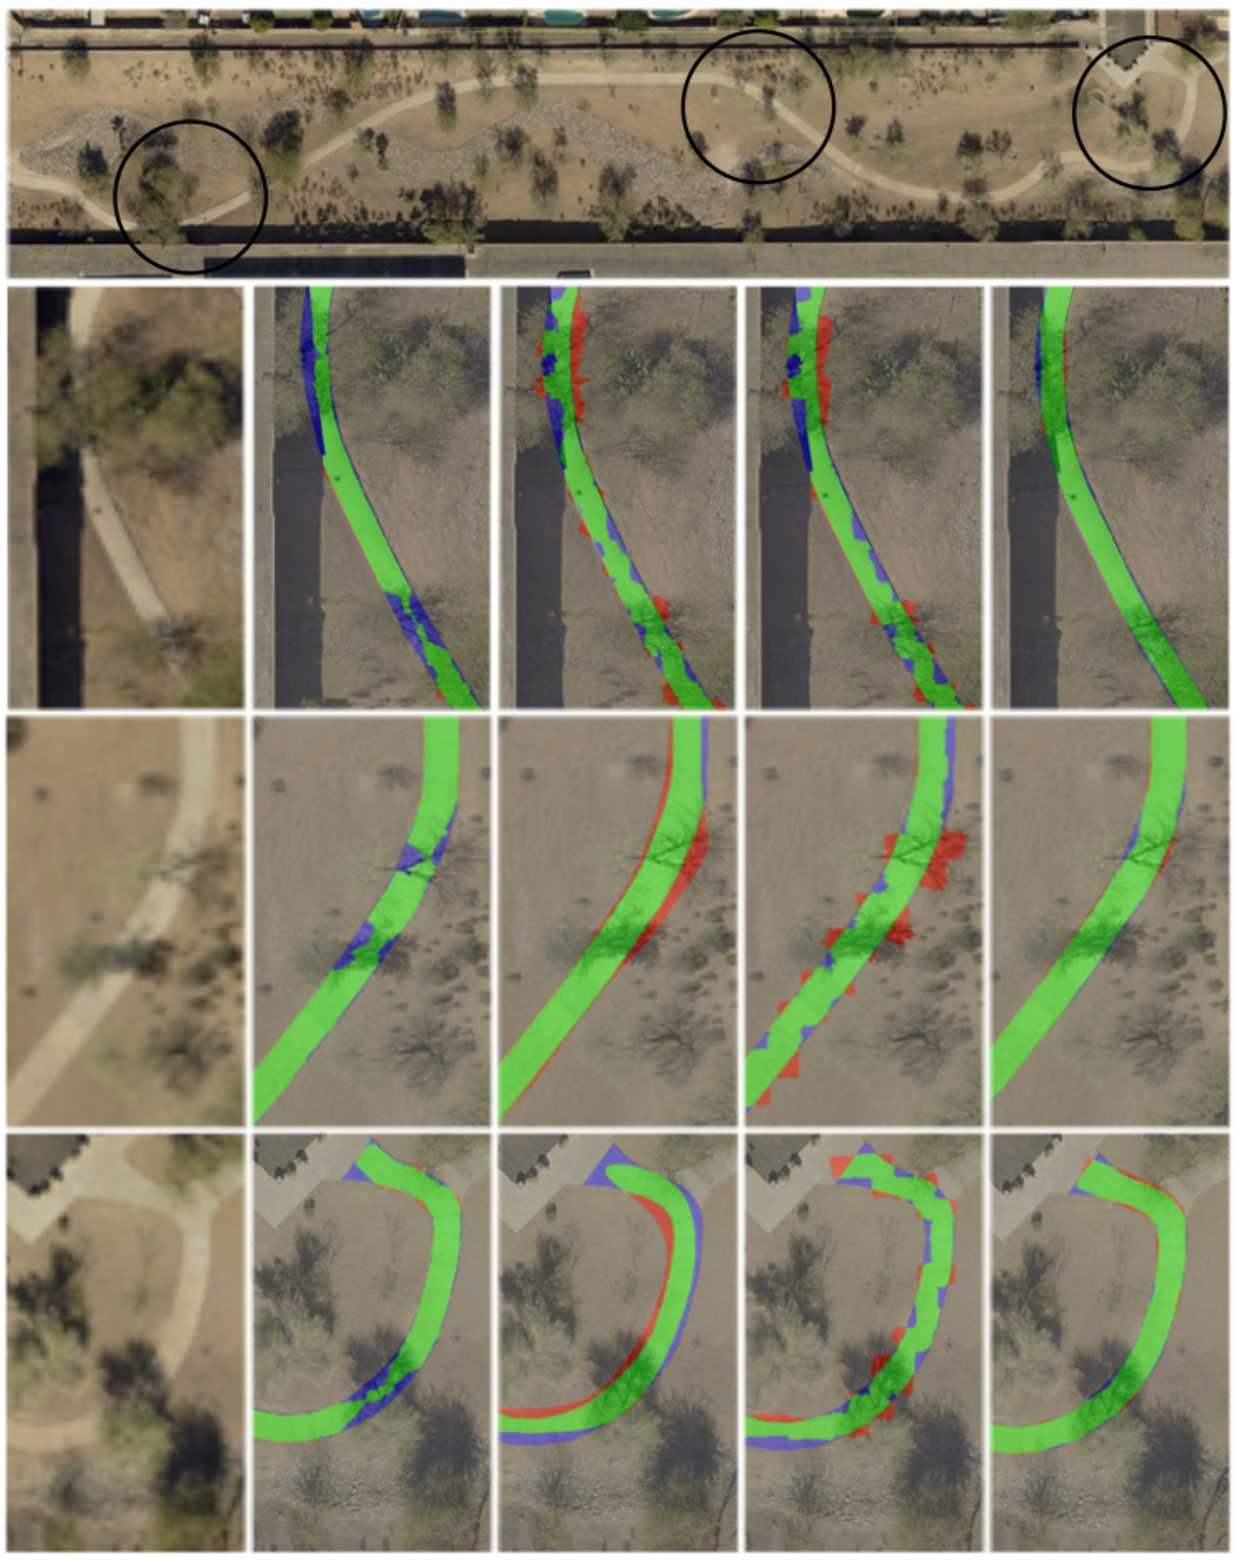
\includegraphics[width=0.9\textwidth]{Figures/4_comparison.pdf}
    \caption[Methods Comparison on Sample Sidewalk 1]{A sample result compared with three different methods and ours. In the order of grabcut, slic, active Contours and ours from left to right. Grabcut is unable to separate the tree shadow from actual sidewalk feature, same with slic and active contours. Our results are more likely to predict the accurate edges under obstacles.}
    \label{fig:Sample_4_compare}
\end{figure}

% \begin{table}[h]
% 	\centering
% 	\begin{tabular}{ | c | c | c | c | } 
% 		\hline
% 		Methods	& TP-FP\% & TP\% & FP\% \\
% 		\hline
% 		Grabcut			& 86.10\% & 87.69\% & 1.82\% \\
% 		\hline
% 		Slic			& 73.90\% & 83.88\% & 11.90\% \\
% 		\hline
% 		Active Contour	& 75.70\% & 86.63\% & 12.63\% \\
% 		\hline
% 		Ours            & 93.48\% & 96.06\% & 2.69\% \\
% 		\hline
% 	\end{tabular}
% 	\caption{Mathematics result comparison between our result and others from figure \ref{fig:Sample_4_compare}}
% 	\label{table:sample_4}	
% \end{table}

\begin{figure}[H]
    \centering
    \includegraphics[width=0.78\textwidth]{Figures/sample_sidewalk_1.png}
    \caption[Methods Comparison on Sample Sidewalk 2]{A sample results compared with three different methods and ours. In the order of active Contours, grabcut, slic, ours from left to right. Which shows samples of separating drive way and gutters.}
    \label{fig:Sample_2_compare}
\end{figure}

\begin{figure}[H]
    \centering
    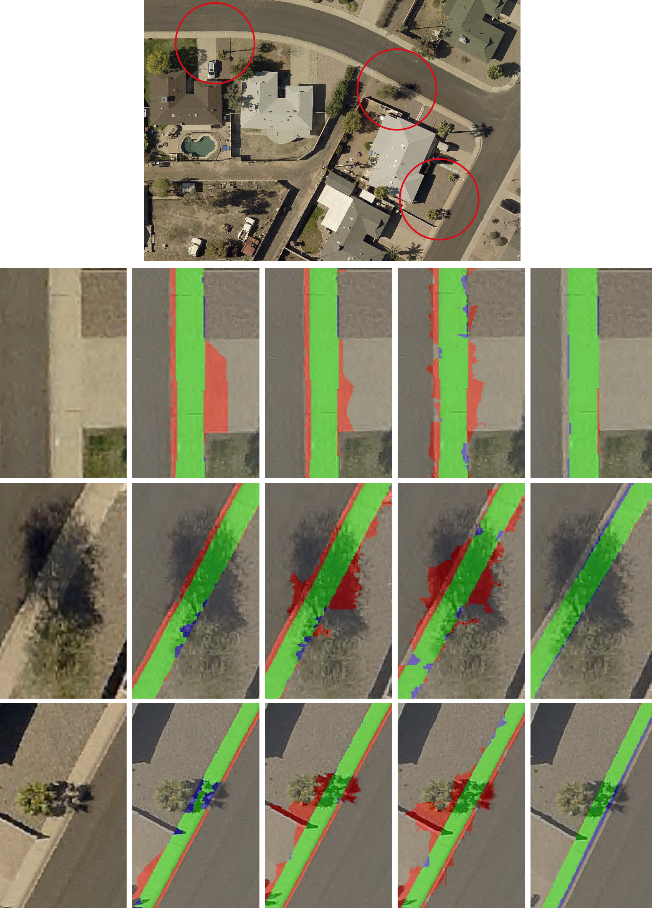
\includegraphics[width=0.86\textwidth]{Figures/2_comparison_needed.png}
    \caption[Methods Comparison on Sample Sidewalk 3]{A sample results compared with three different methods and ours. In the order of grabcut, slic, active Contours, ours from left to right. Which shows samples of separating drive way and gutters.}
    \label{fig:Sample_3_compare}
\end{figure}



\begin{figure}[H]
    \centering
    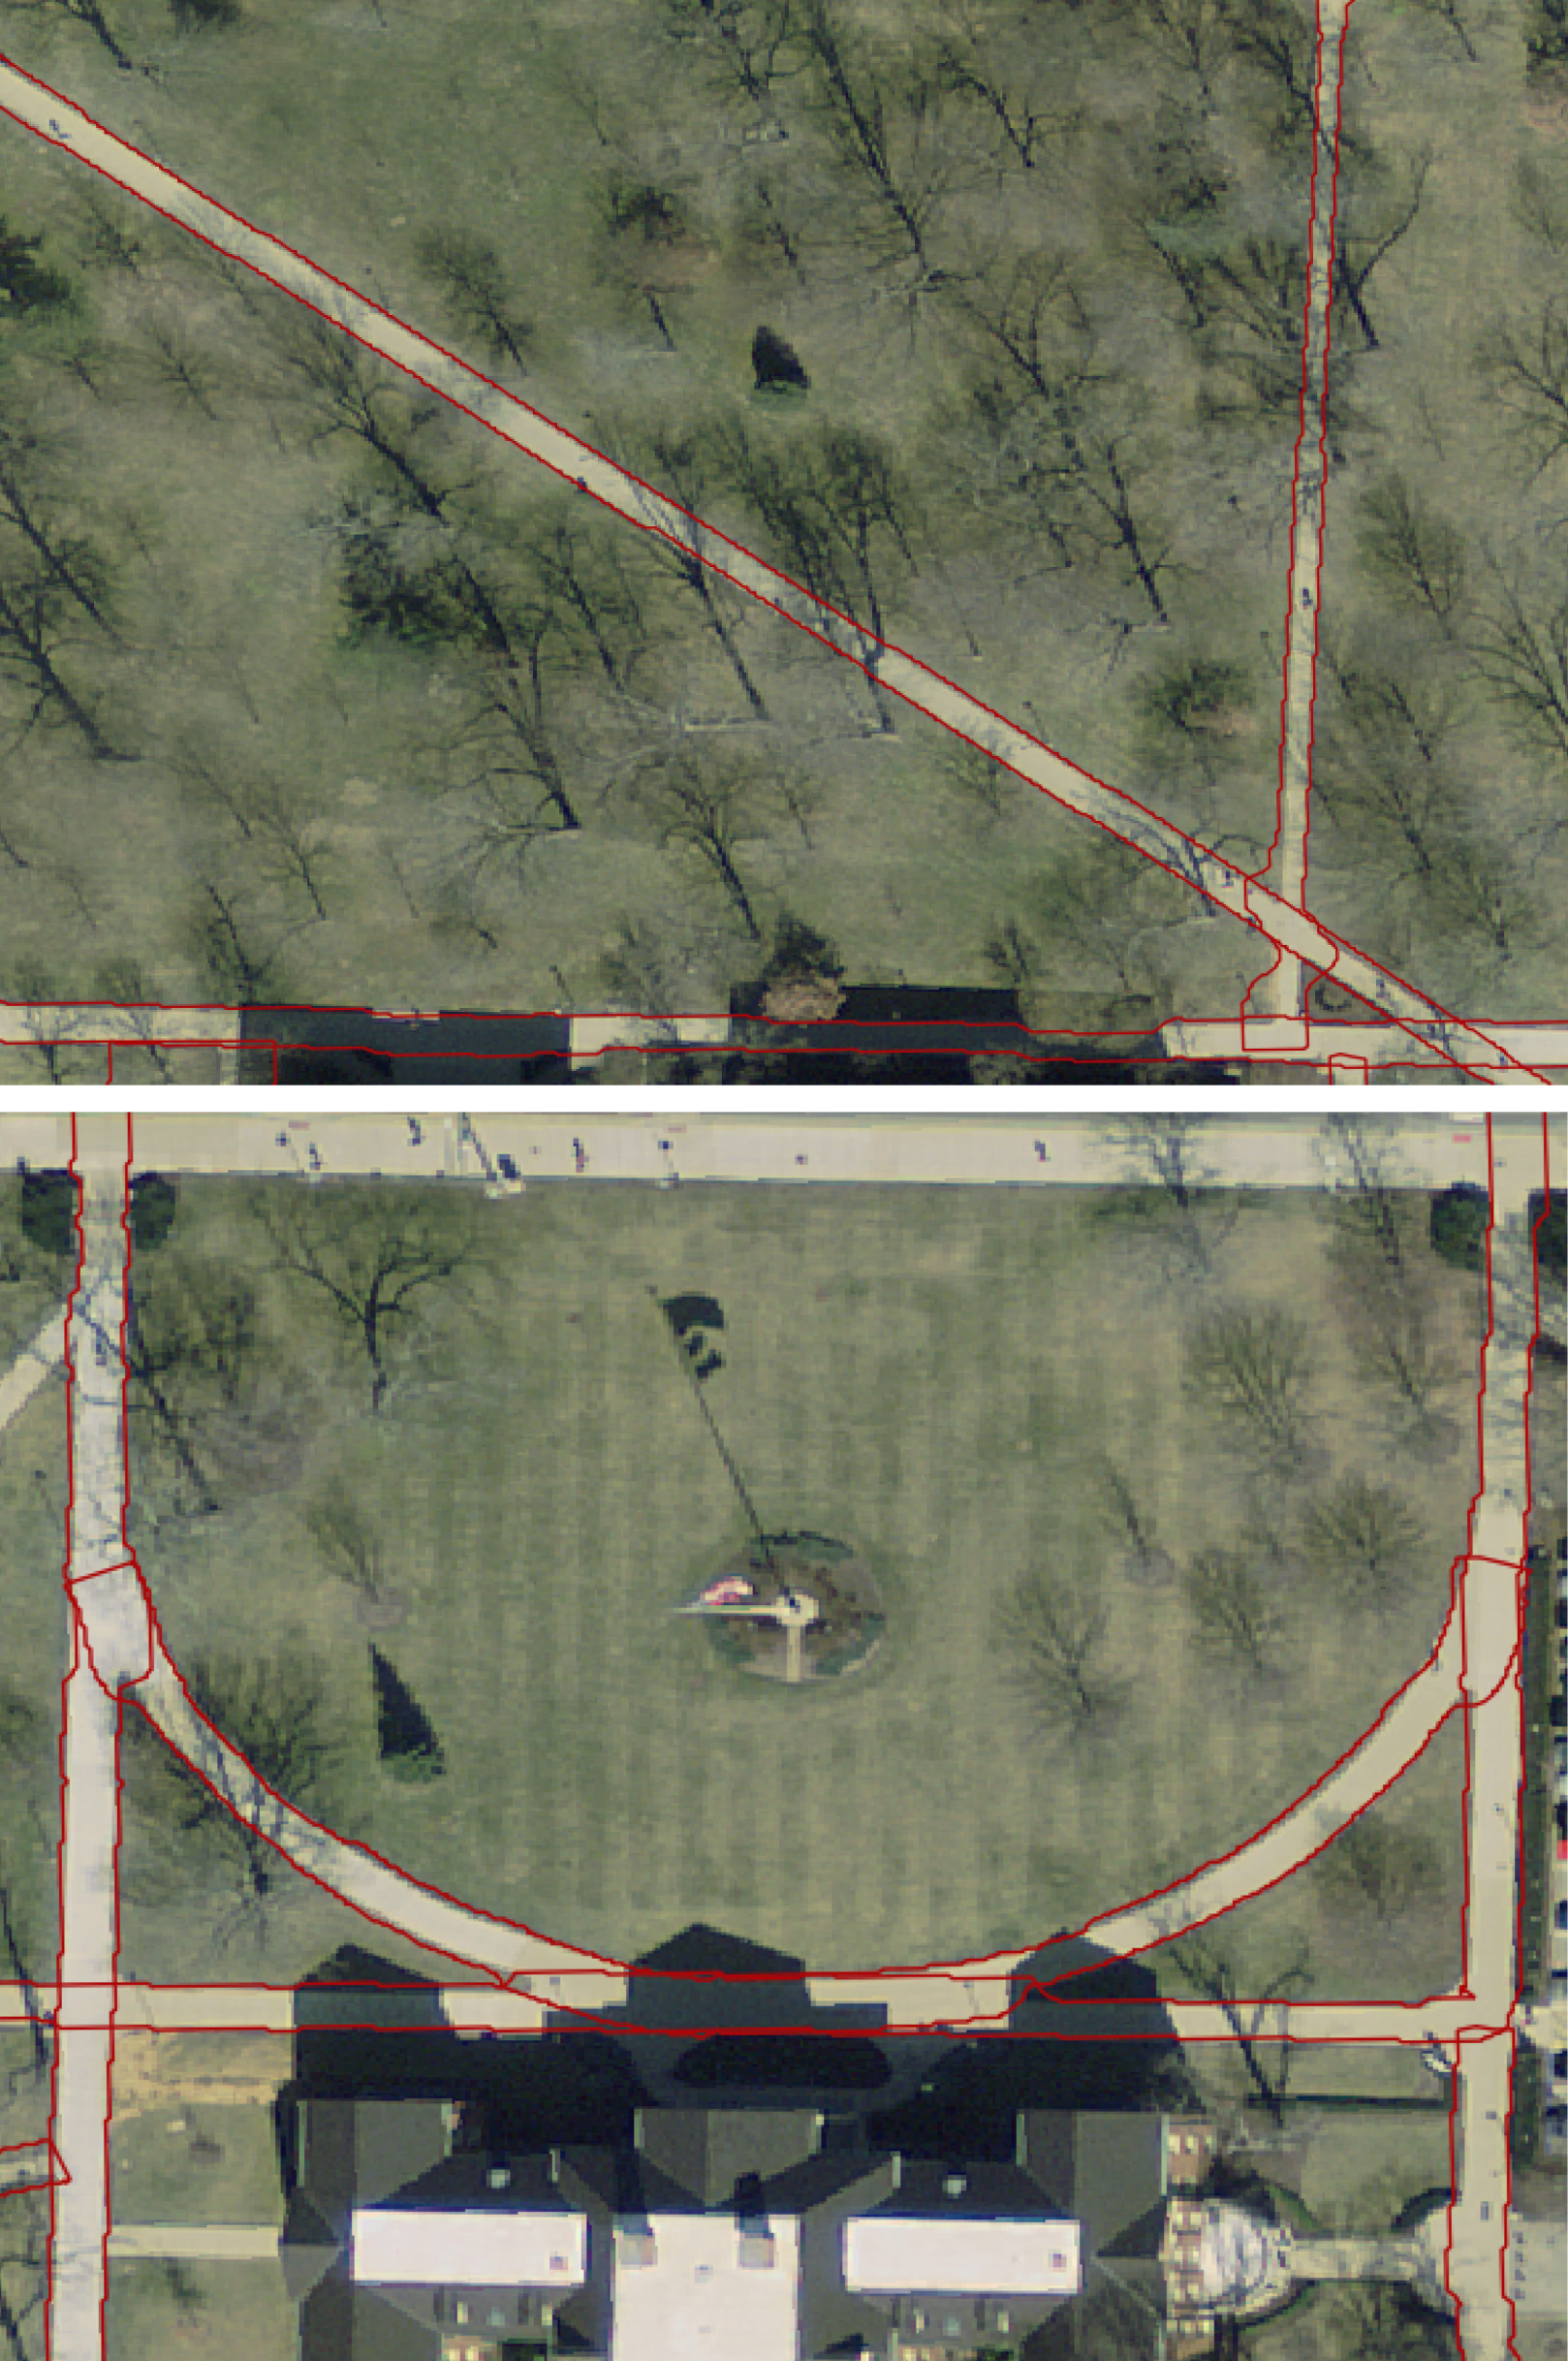
\includegraphics[width=0.8\textwidth]{Figures/Oxford_success_complex.png}
    \caption[Sample Sidewalk 3]{Demonstration on sample sidewalks with our approach. We use Oxford Area that include more complex sidewalks. It shows that given samples are able to separate trees, building shadows and camouflage with adjacent materials.}
    \label{fig:oxford1}
\end{figure}

\begin{figure}[H]
    \centering
    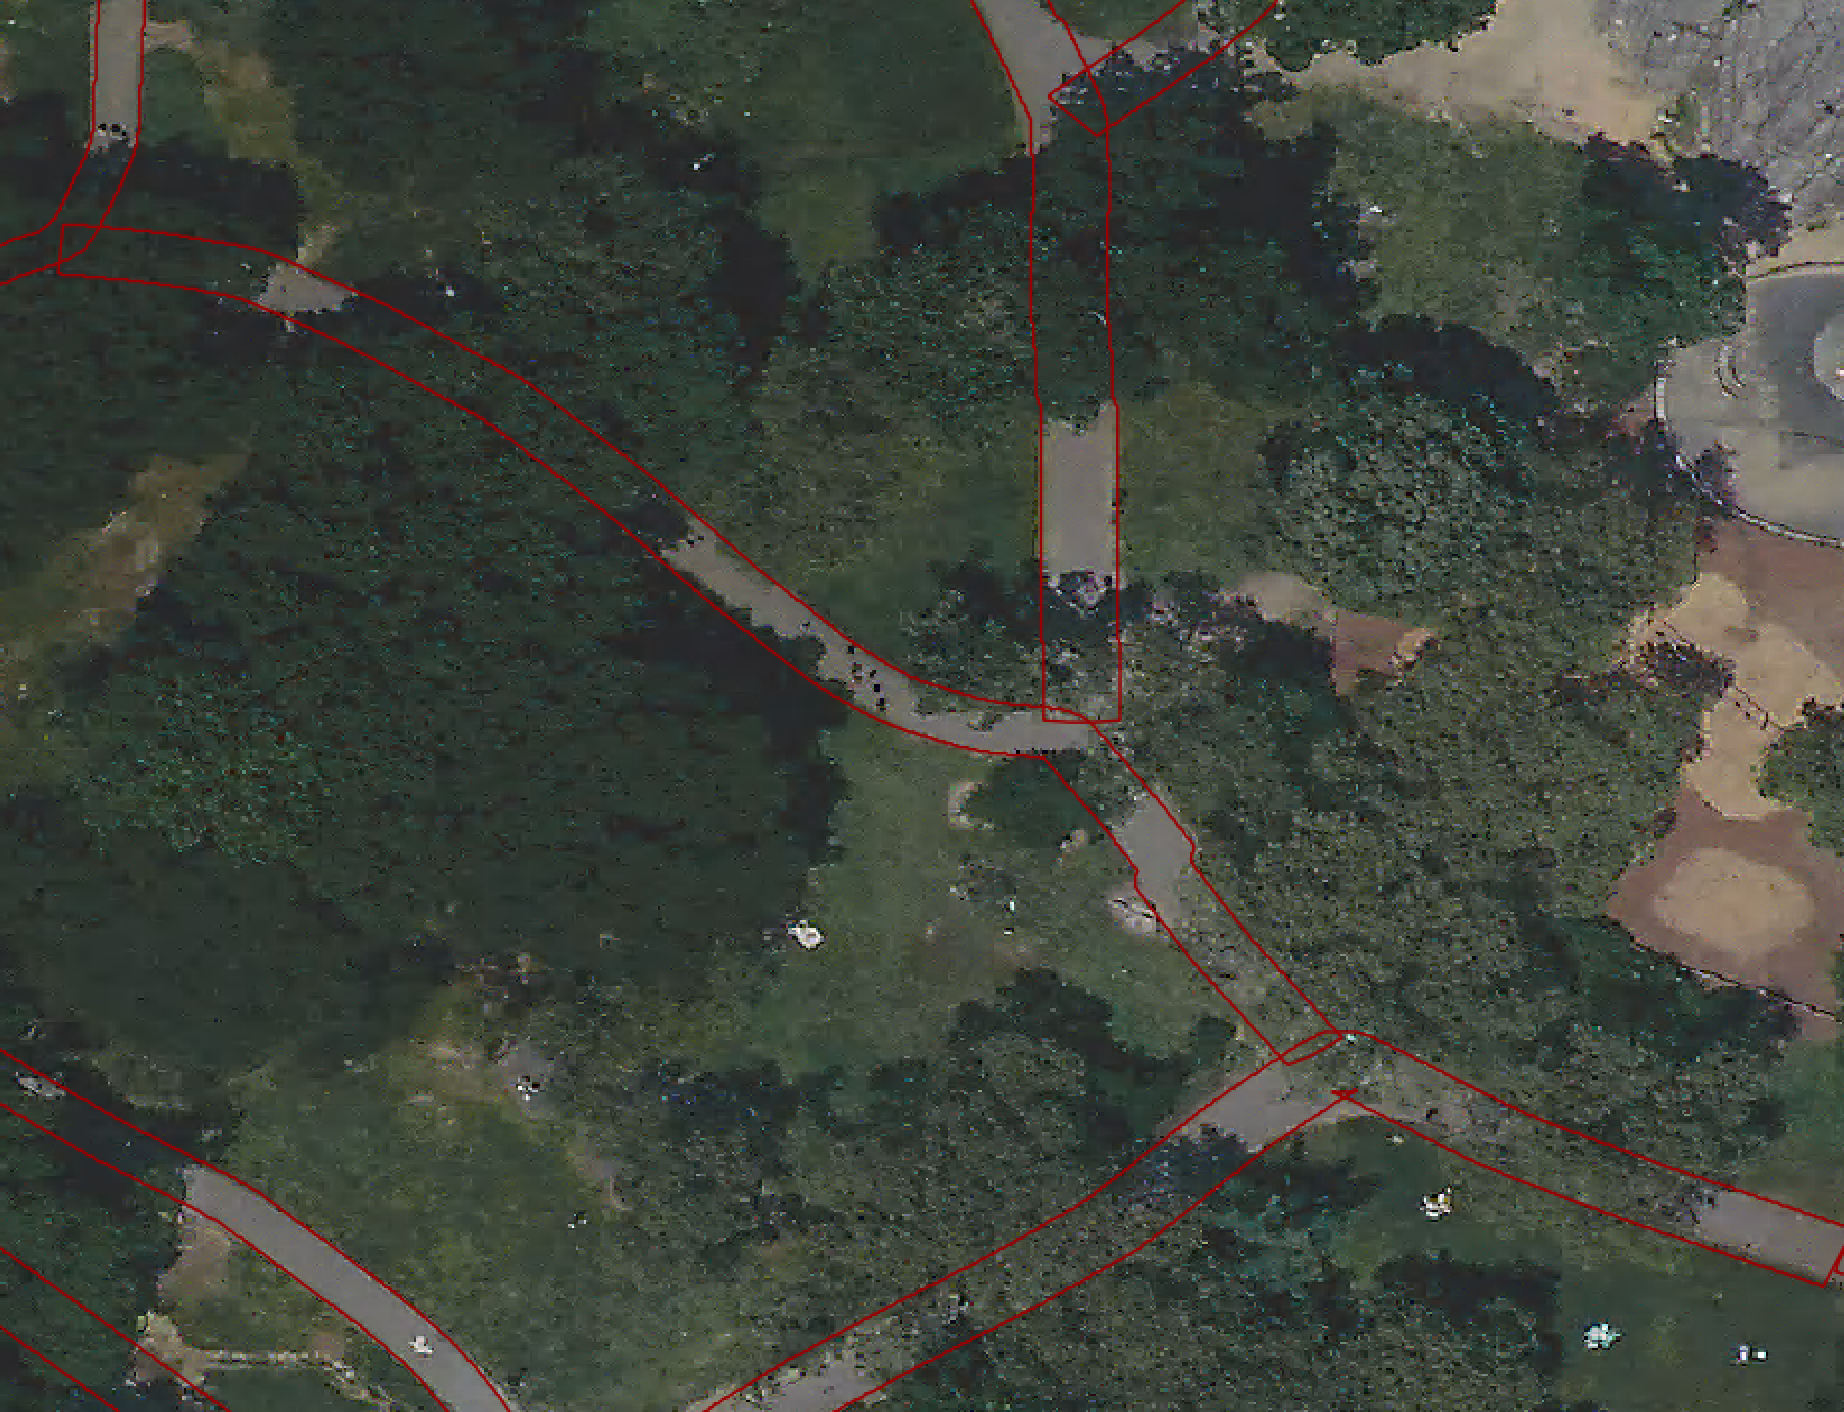
\includegraphics[width=\textwidth]{Figures/ny1.png}
    \caption[Sample Sidewalk 4]{Demonstration on sample sidewalks with our approach. We use New York area that include more complex sidewalks. Our approach is able to separate tree shadows and obstacles. It also has a decent performance on predicating boundaries on partial sidewalks that are fully covered by tree leaves.}
    \label{fig:ny1}
\end{figure}

% \begin{figure}
%     \centering
%     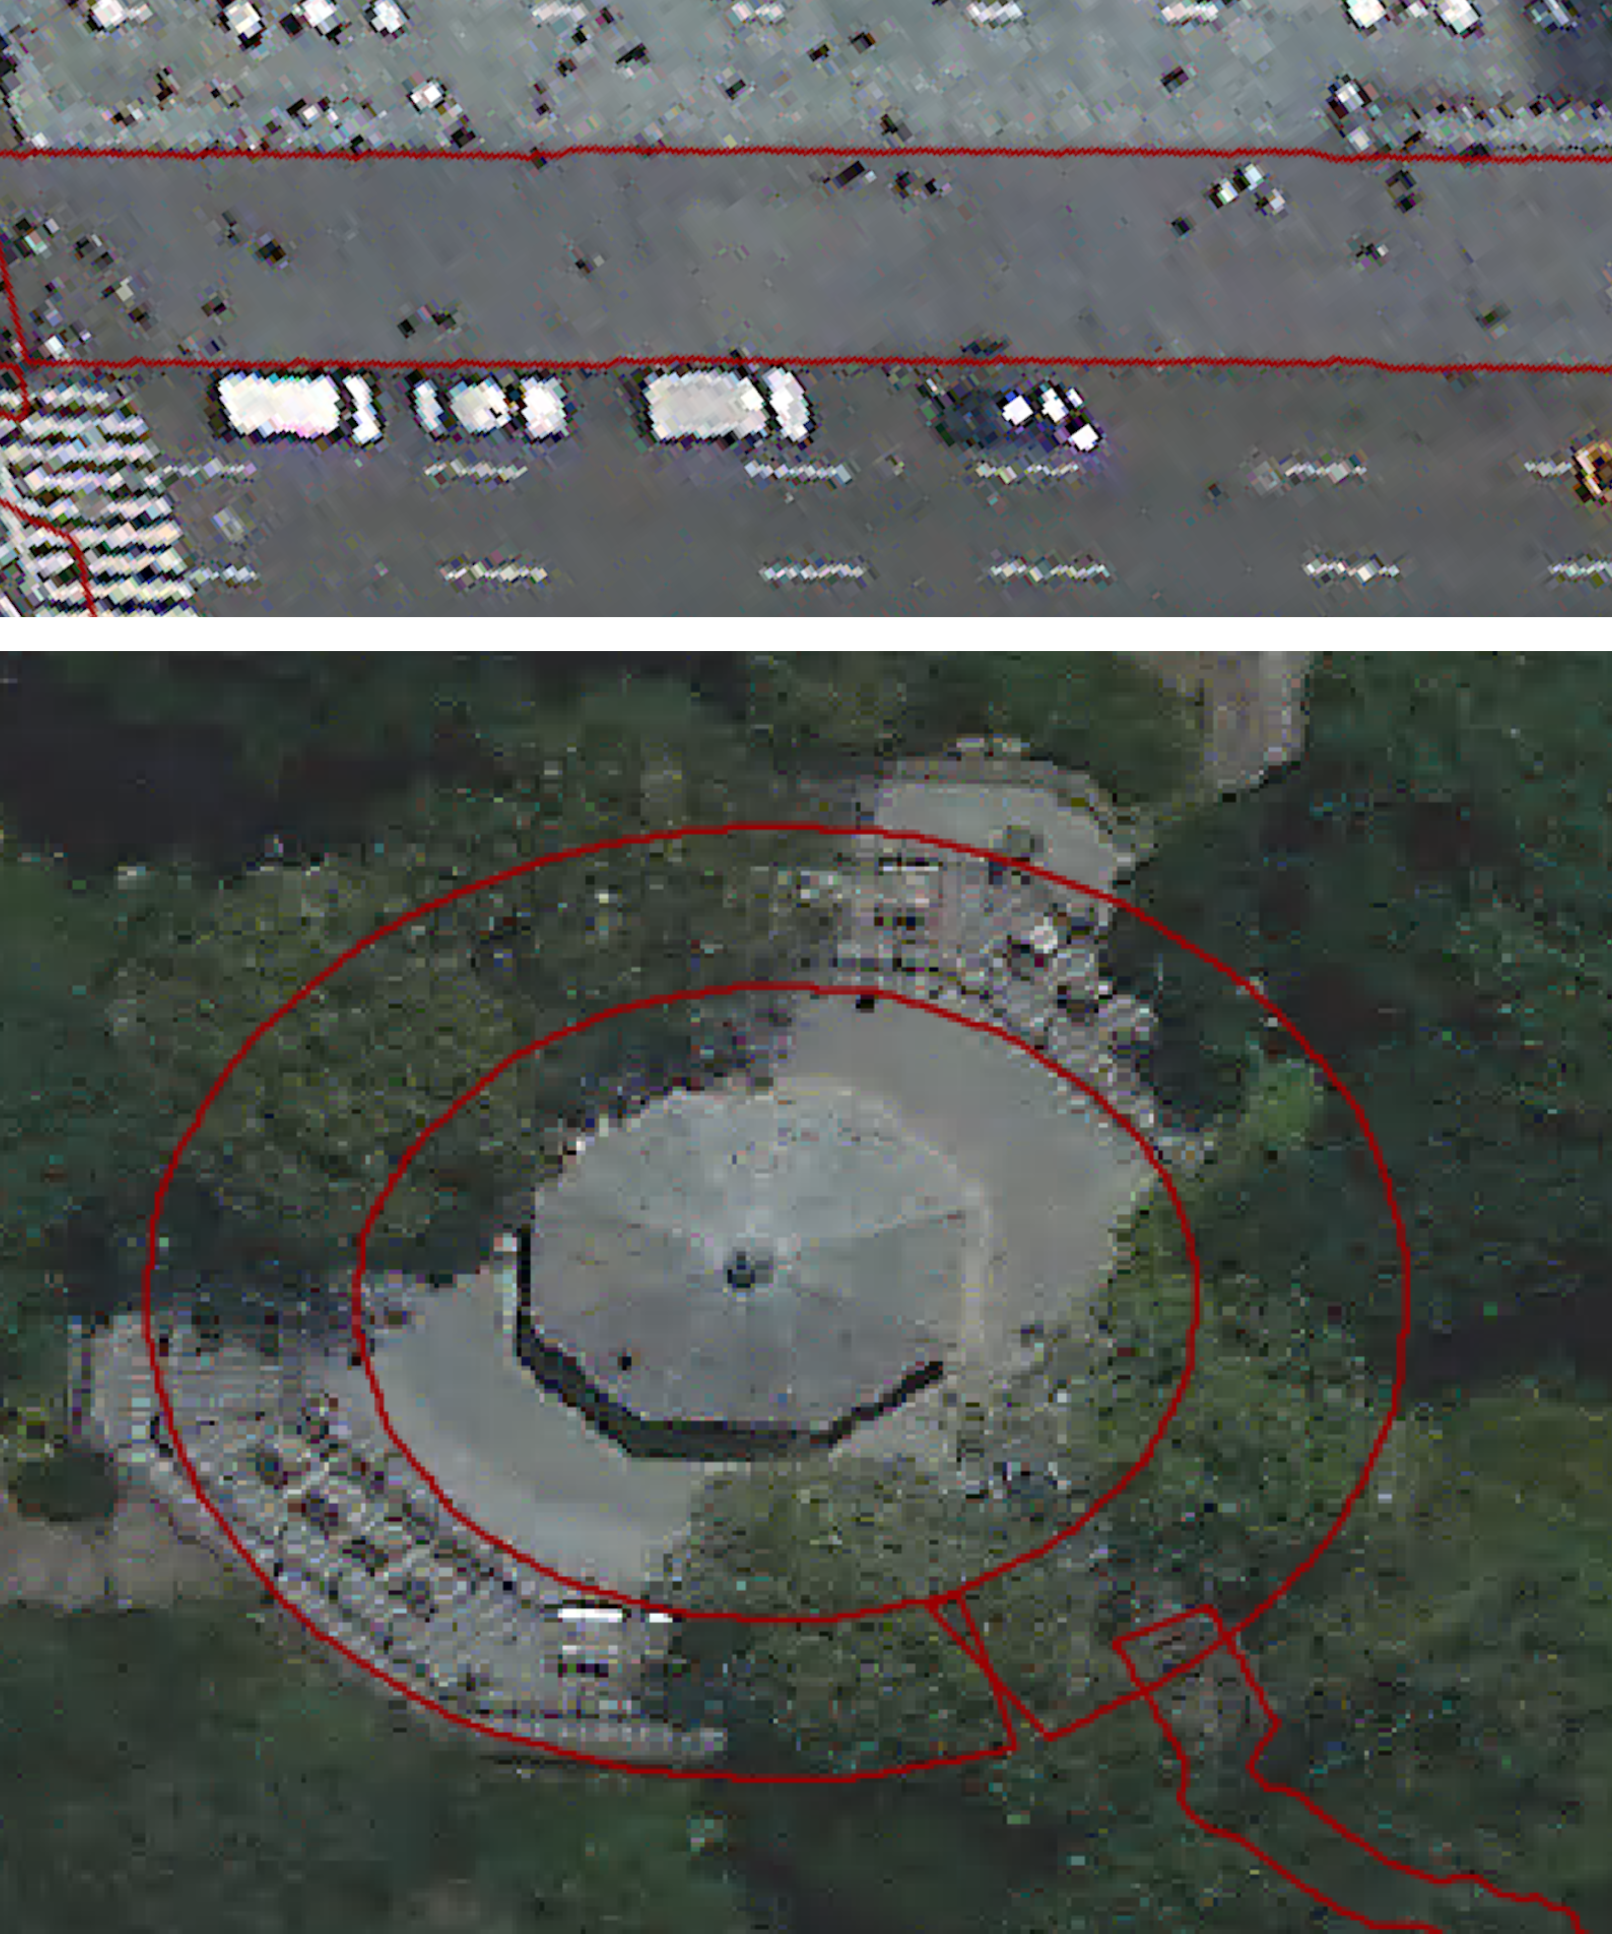
\includegraphics[width=\textwidth]{Figures/ny2.png}
%     \caption[Sample Sidewalk 5]{Demonstration on sample sidewalks with our approach. We use sidewalks that are random selected from New York area. Row 1 shows a thicker sidewalk that camouflage with adjacent road and street. Row 2 shows complex sidewalk texture with irregular shape.}
%     \label{fig:ny2}
% \end{figure}

\begin{figure}[H]
    \centering
    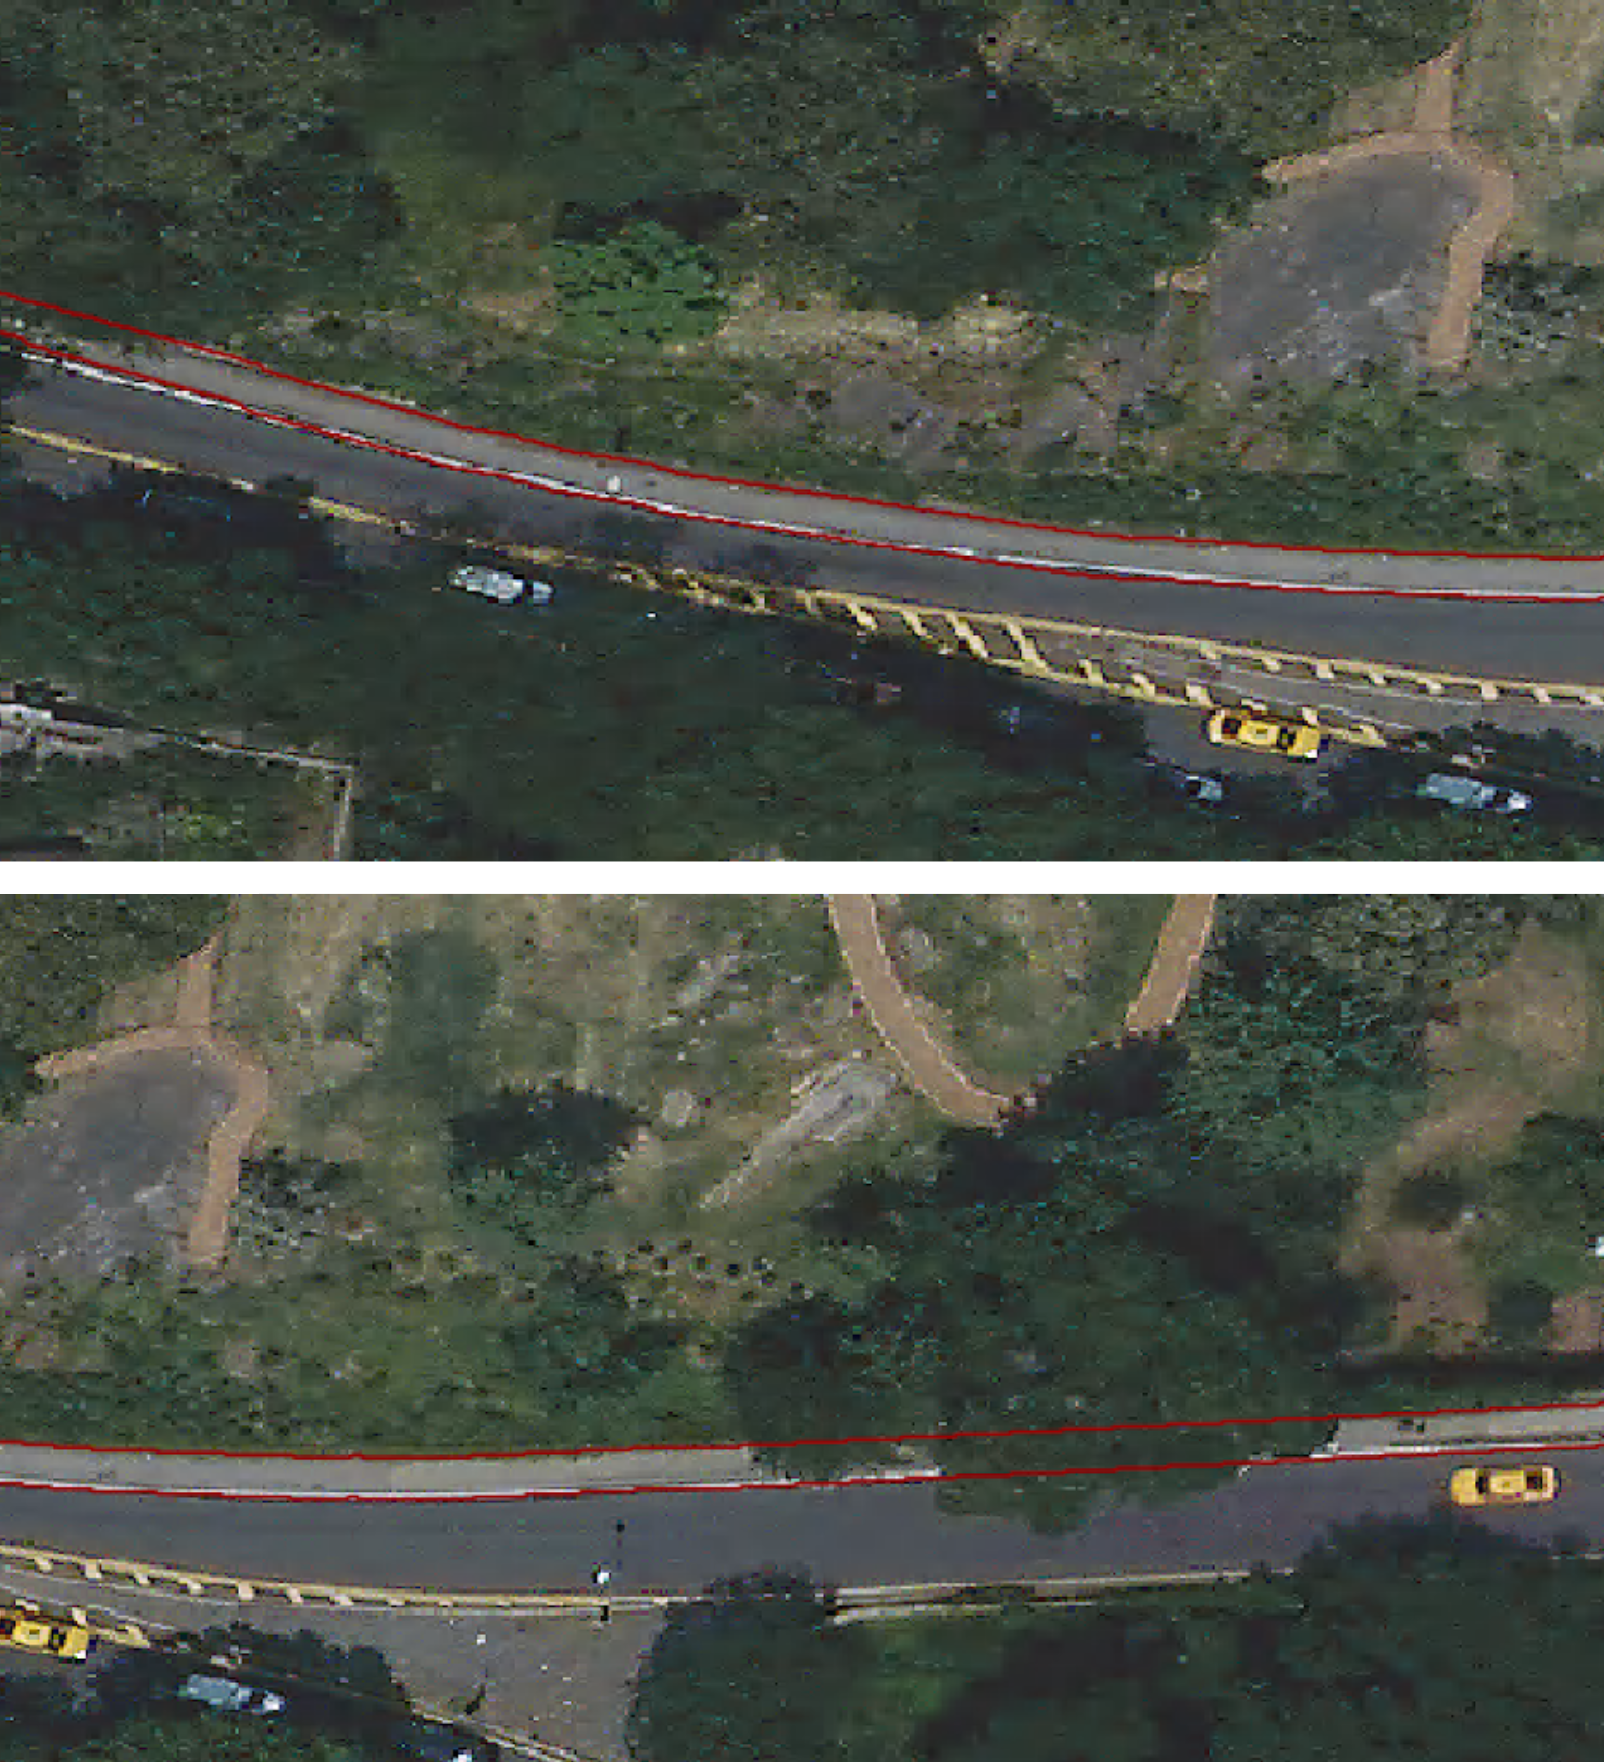
\includegraphics[width=\textwidth]{Figures/ny3.png}
    \caption[Sample Sidewalk 6]{Demonstration on sample sidewalks with our approach. It shows a continues site but we separate it due to it's length. Our approach did recognized the sidewalk part under the tree top and predict it's precise boundaries.}
    \label{fig:ny3}
\end{figure}

\section{Failure Cases}

We produce some failure cases to show what we need to improve for the future work. 

\begin{enumerate}
    \item Miss matching data set: Figure \ref{fig:oxford_fail_1} shows the failure case when the input map data and the trajectory data not match. The map data is older than the trajectory data, so the boundaries we generated is not yet existed on the map. Since the road structures changes over time, it's possible to get the data set in different time stamp. 
    \item Irregular Intersections: Figure \ref{fig:oxford_fail_2} shows the failure case when process irregular shape intersections. Our approach is able to generate the boundaries when the sidewalk is able to reshape into ribbon-image. Such as in figure \ref{fig:oxford_fail_2}, it's not yet able to produce the sidewalk boundaries with irregular shape intersection.
    \item Fully blocked sidewalk: \figref{fig:ny_fail_1} shows sample of sidewalks that fully blocked by obstacles, tree crown in our case. Base on the initial trajectory we find from open source, there must be a sidewalk under the tree crown. We count this as 'failure' cases since it's impossible for us to determine the accuracy for our result. 
\end{enumerate}

\begin{figure}[H]
    \centering
    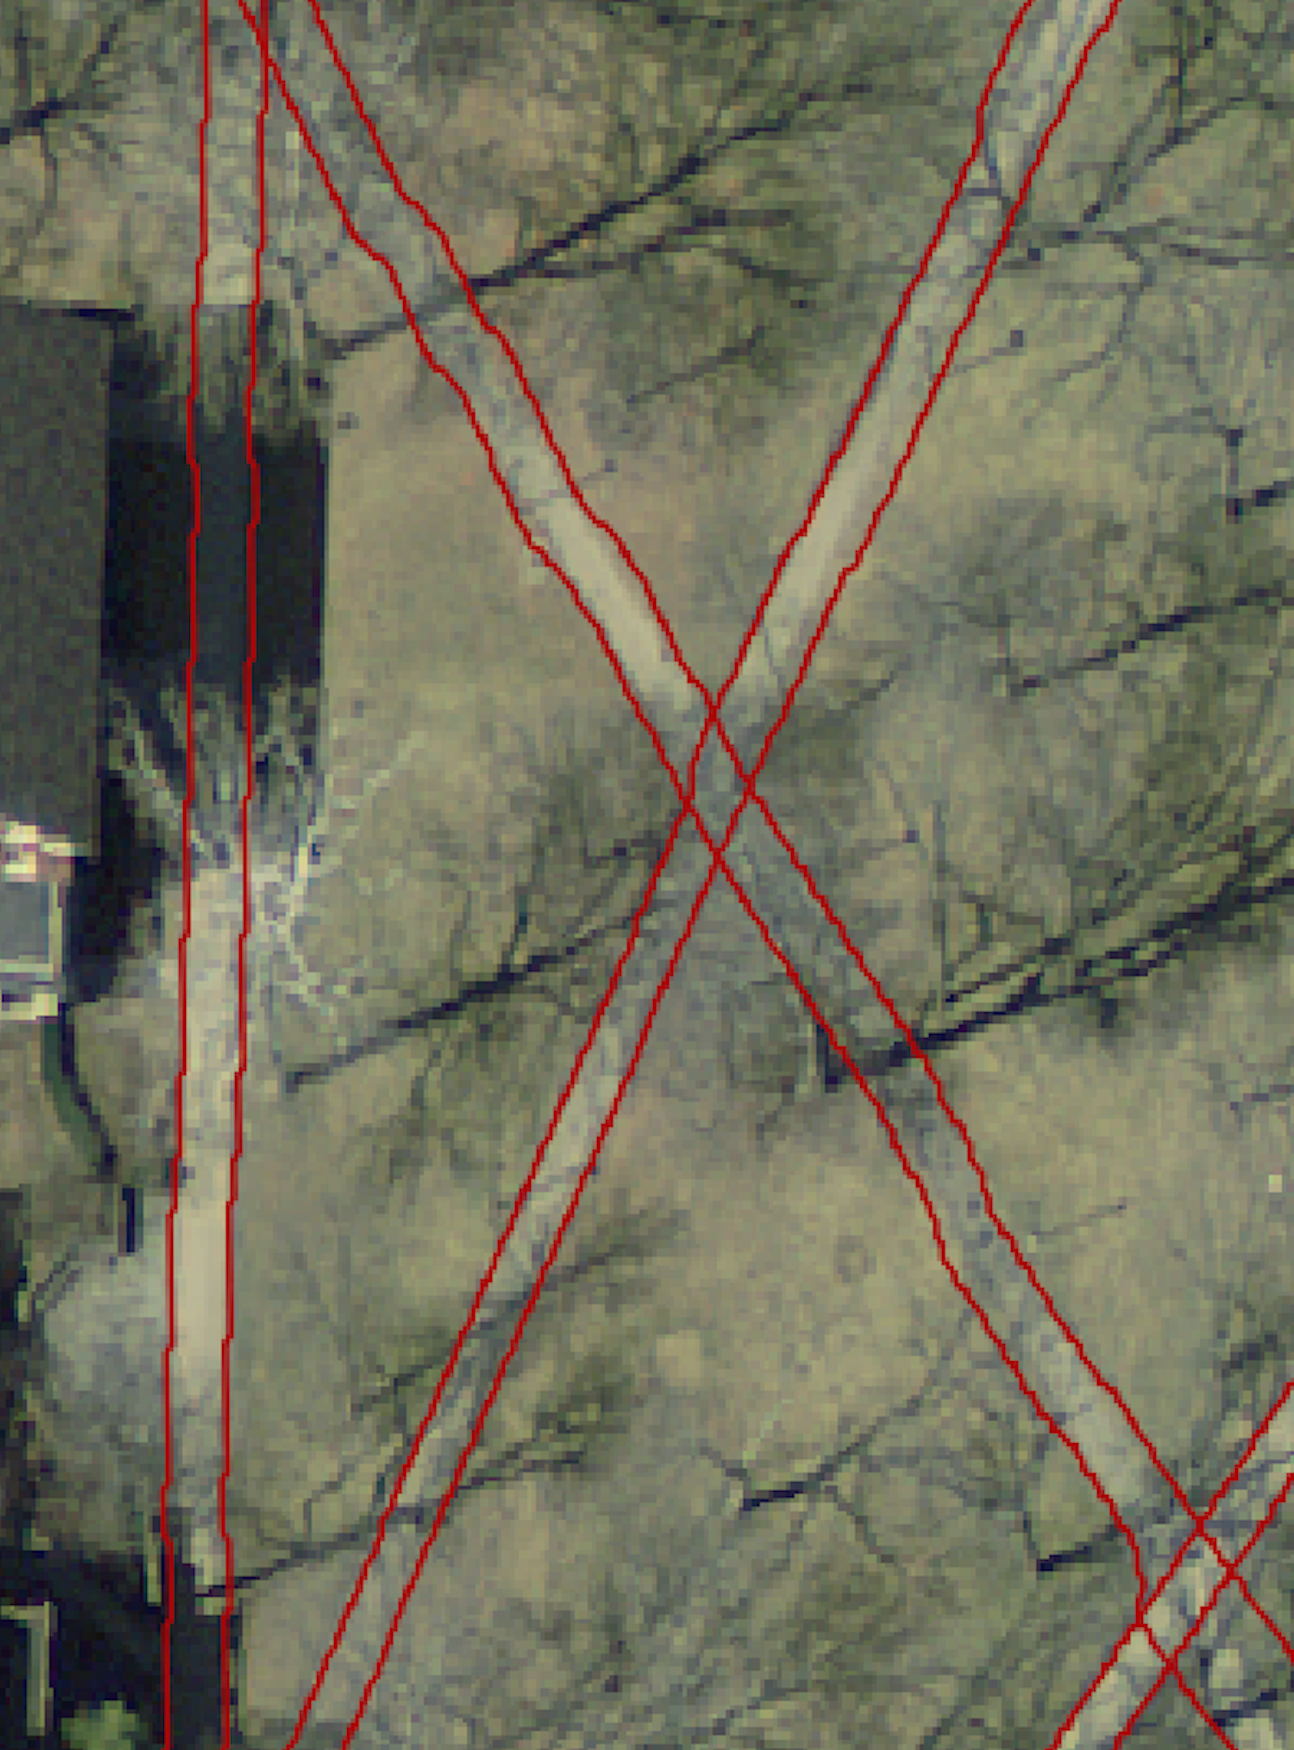
\includegraphics[width=0.83\textwidth]{Figures/oxford_fail_1.png}
    \caption[Failure Case 1]{Demonstration on failure cases. Due to the fact that road structures may change overtime. It's possible to produce the output with the input map and the initial trajectory within different time stamp. Sample figure shows our approach produce 'incorrect' sidewalk boundaries because the map data is older than the trajectory so we are producing the sidewalk that were not built yet.}
    \label{fig:oxford_fail_1}
\end{figure} 

\begin{figure}
    \centering
    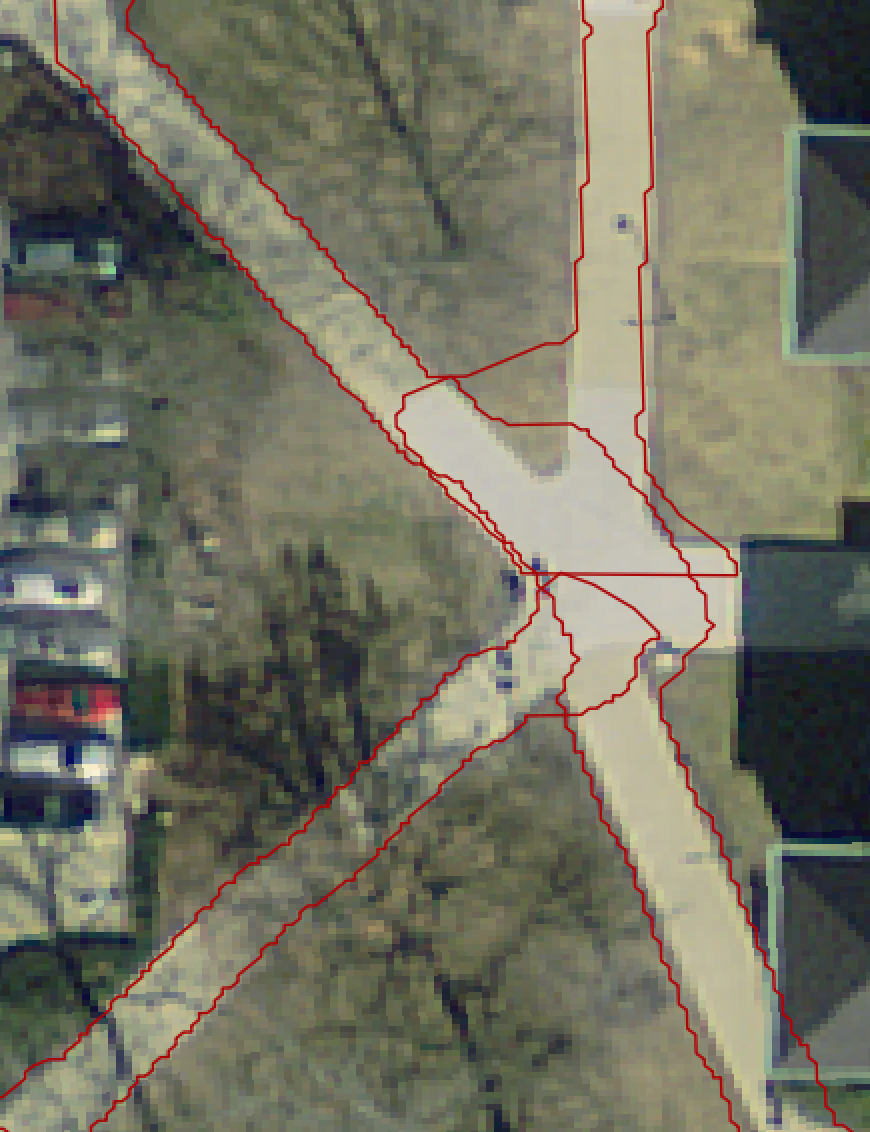
\includegraphics[width=0.9\textwidth]{Figures/oxford_fail_2.png}
    \caption[Failure Case 2]{Demonstration on failure cases. Our approach was developed to produce boundaries for single sidewalk, and it's not yet able to process intersection with irregular shape.}
    \label{fig:oxford_fail_2}
\end{figure} 

\begin{figure}
    \centering
    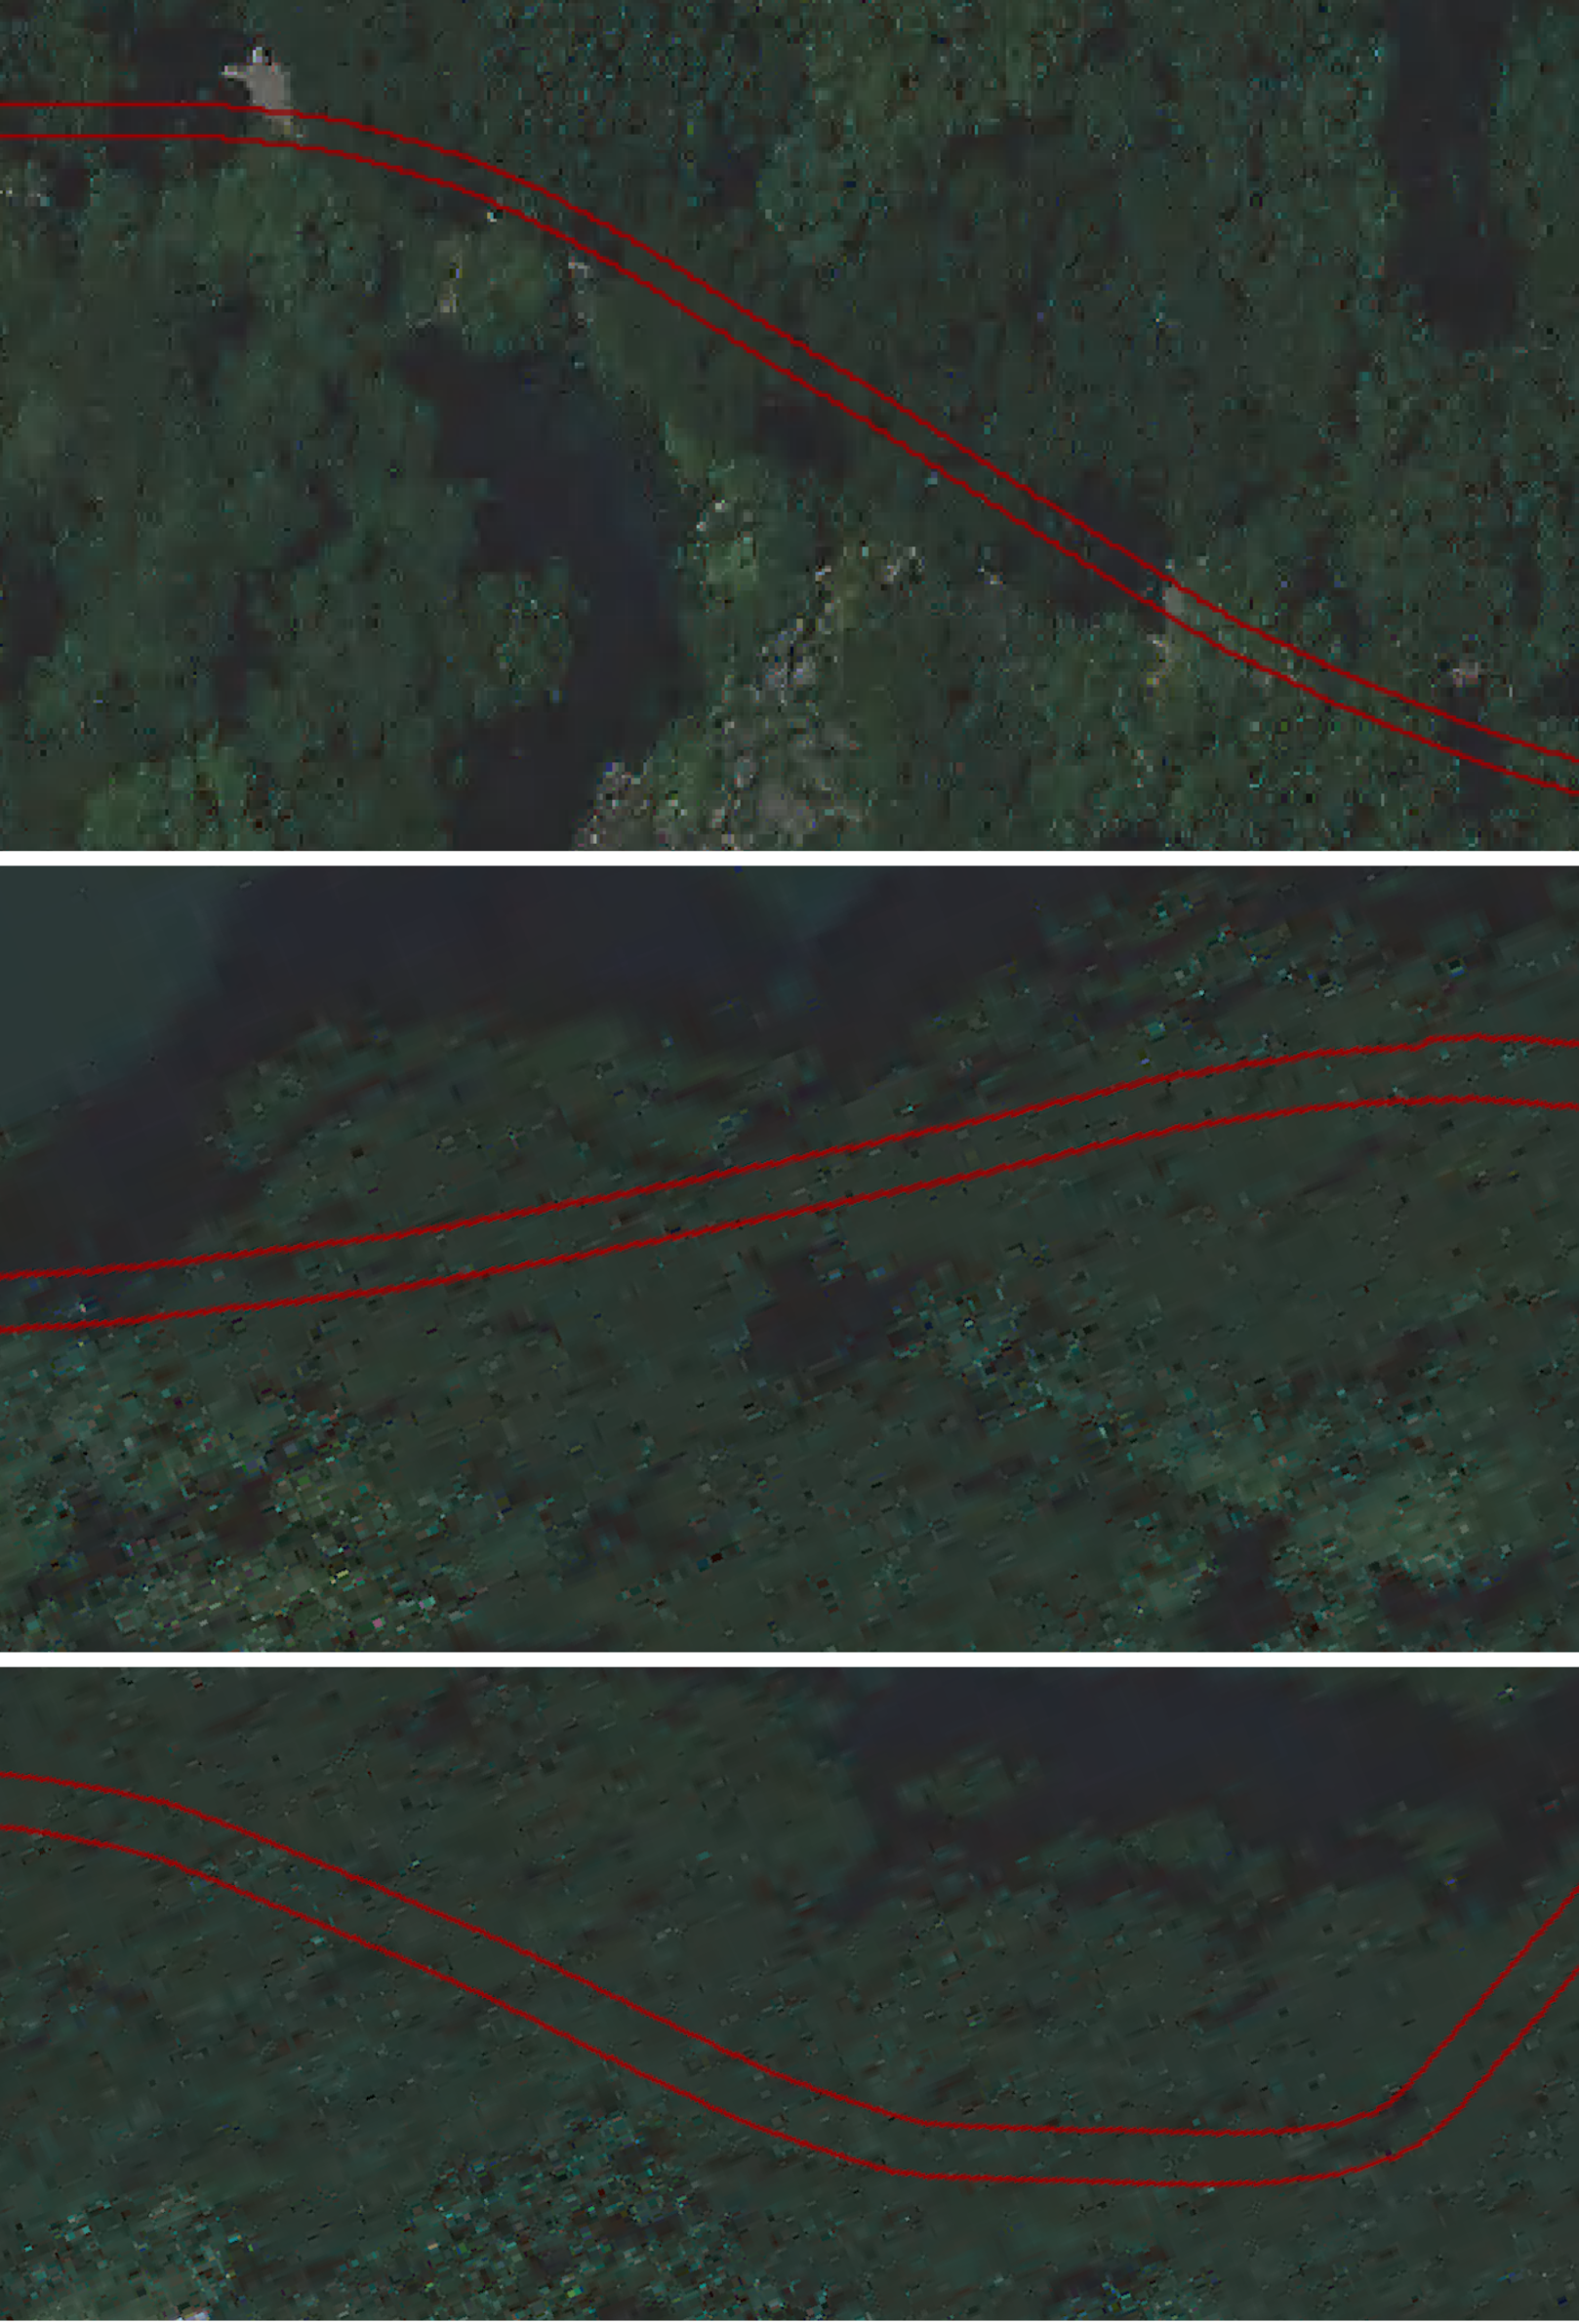
\includegraphics[width=0.8\textwidth]{Figures/ny_failcase.png}
    \caption[Failure Case 3]{Demonstration on failure cases. Our approach is not able to determine the sidewalk boundaries that's completely blocked by obstacles. The result is base on the average of sidewalks width but it's impossible for us to compare the prediction with accurate result.}
    \label{fig:ny_fail_1}
\end{figure} 

\section{Future Work}

There's couple more ideas we would like to attempt.

\begin{enumerate}
    \item To simplify the process, we would like to generate the sidewalk with just latitudes and longitudes.
    
    we can use the latitudes and longitudes data to locate a part of a map via Overpass Turbo \cite{overpass_turbo}, it supports features such as sidewalks geometric location since it's connecting with the database from \ac{OSM} \cite{OpenStreetMap}. Also, with the input latitudes and longitudes data, we can extract the map with given range from Google map or other open map source. Then just simply pass in both data set with our approach to generate whole sidewalk information for the whole site. 
    
    \item We'll give hypothesis to process the intersection area. We identify the point that is overlapped as intersection part (same node in multiple ways), we connect nodes on each way that are adjacent to the point. By extend each path a little bit more into the adjacent path to finish the intersection. Figure \ref{fig:intersection} shows the basic idea of our hypothesis, the sidewalk from the left merges into the left. It's connecting the left sidewalk into the right one and processed it as the same part. 
    
\end{enumerate}

\begin{figure}
    \centering
    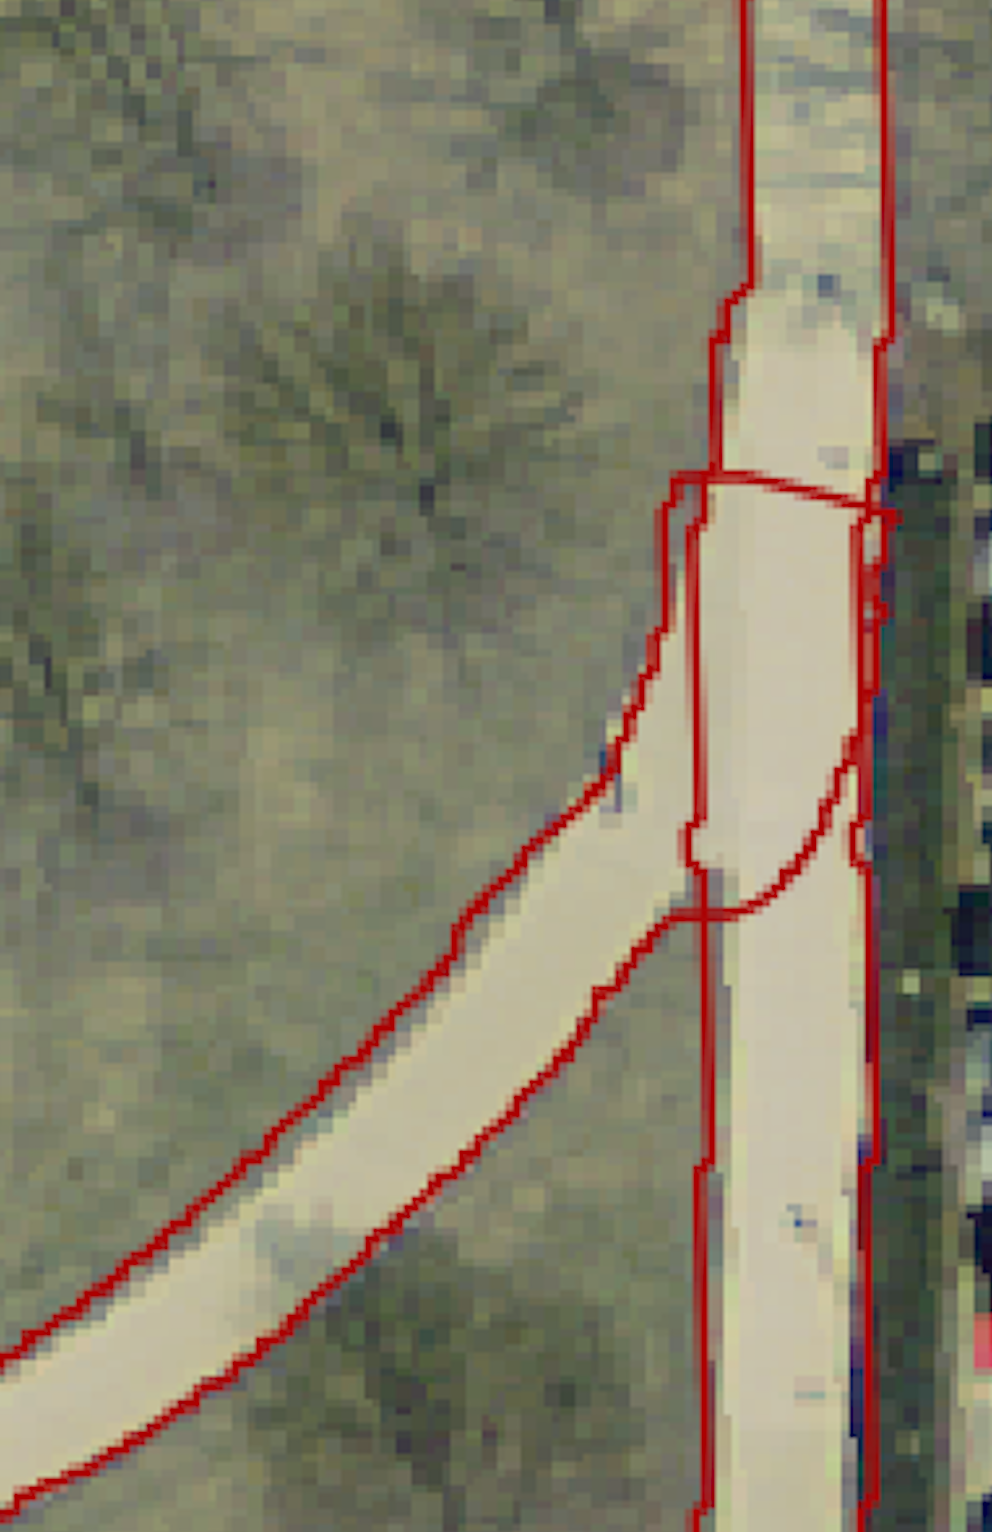
\includegraphics[width=0.75\textwidth]{Figures/intersection.png}
    \caption[Intersection Demonstration]{A hypothesis demonstration on intersection. By extend each path a little bit more into the next adjacent path, we can connect them we a little 'elbow'.}
    \label{fig:intersection}
\end{figure}

